Die Verstärkerelektronik soll zuerst bei Raumtemperatur und Flüssigstickstoff Temperatur getestet werden.
Dabei soll das Rauschen und die Übertragungsfunktion der kalten Elektronik, wie sie in den Abschnitten \ref{sec:Ausleseelektronik} und \ref{sec:Amp} dargestellt ist, bestimmt werden.
Der Versuchsaufbau sollte den Bedingungen, welche beim Einsatz im Kryostaten mit Detektor gegeben sind, möglichst nahe sein.
\begin{figure}[!t]
\begin{center}
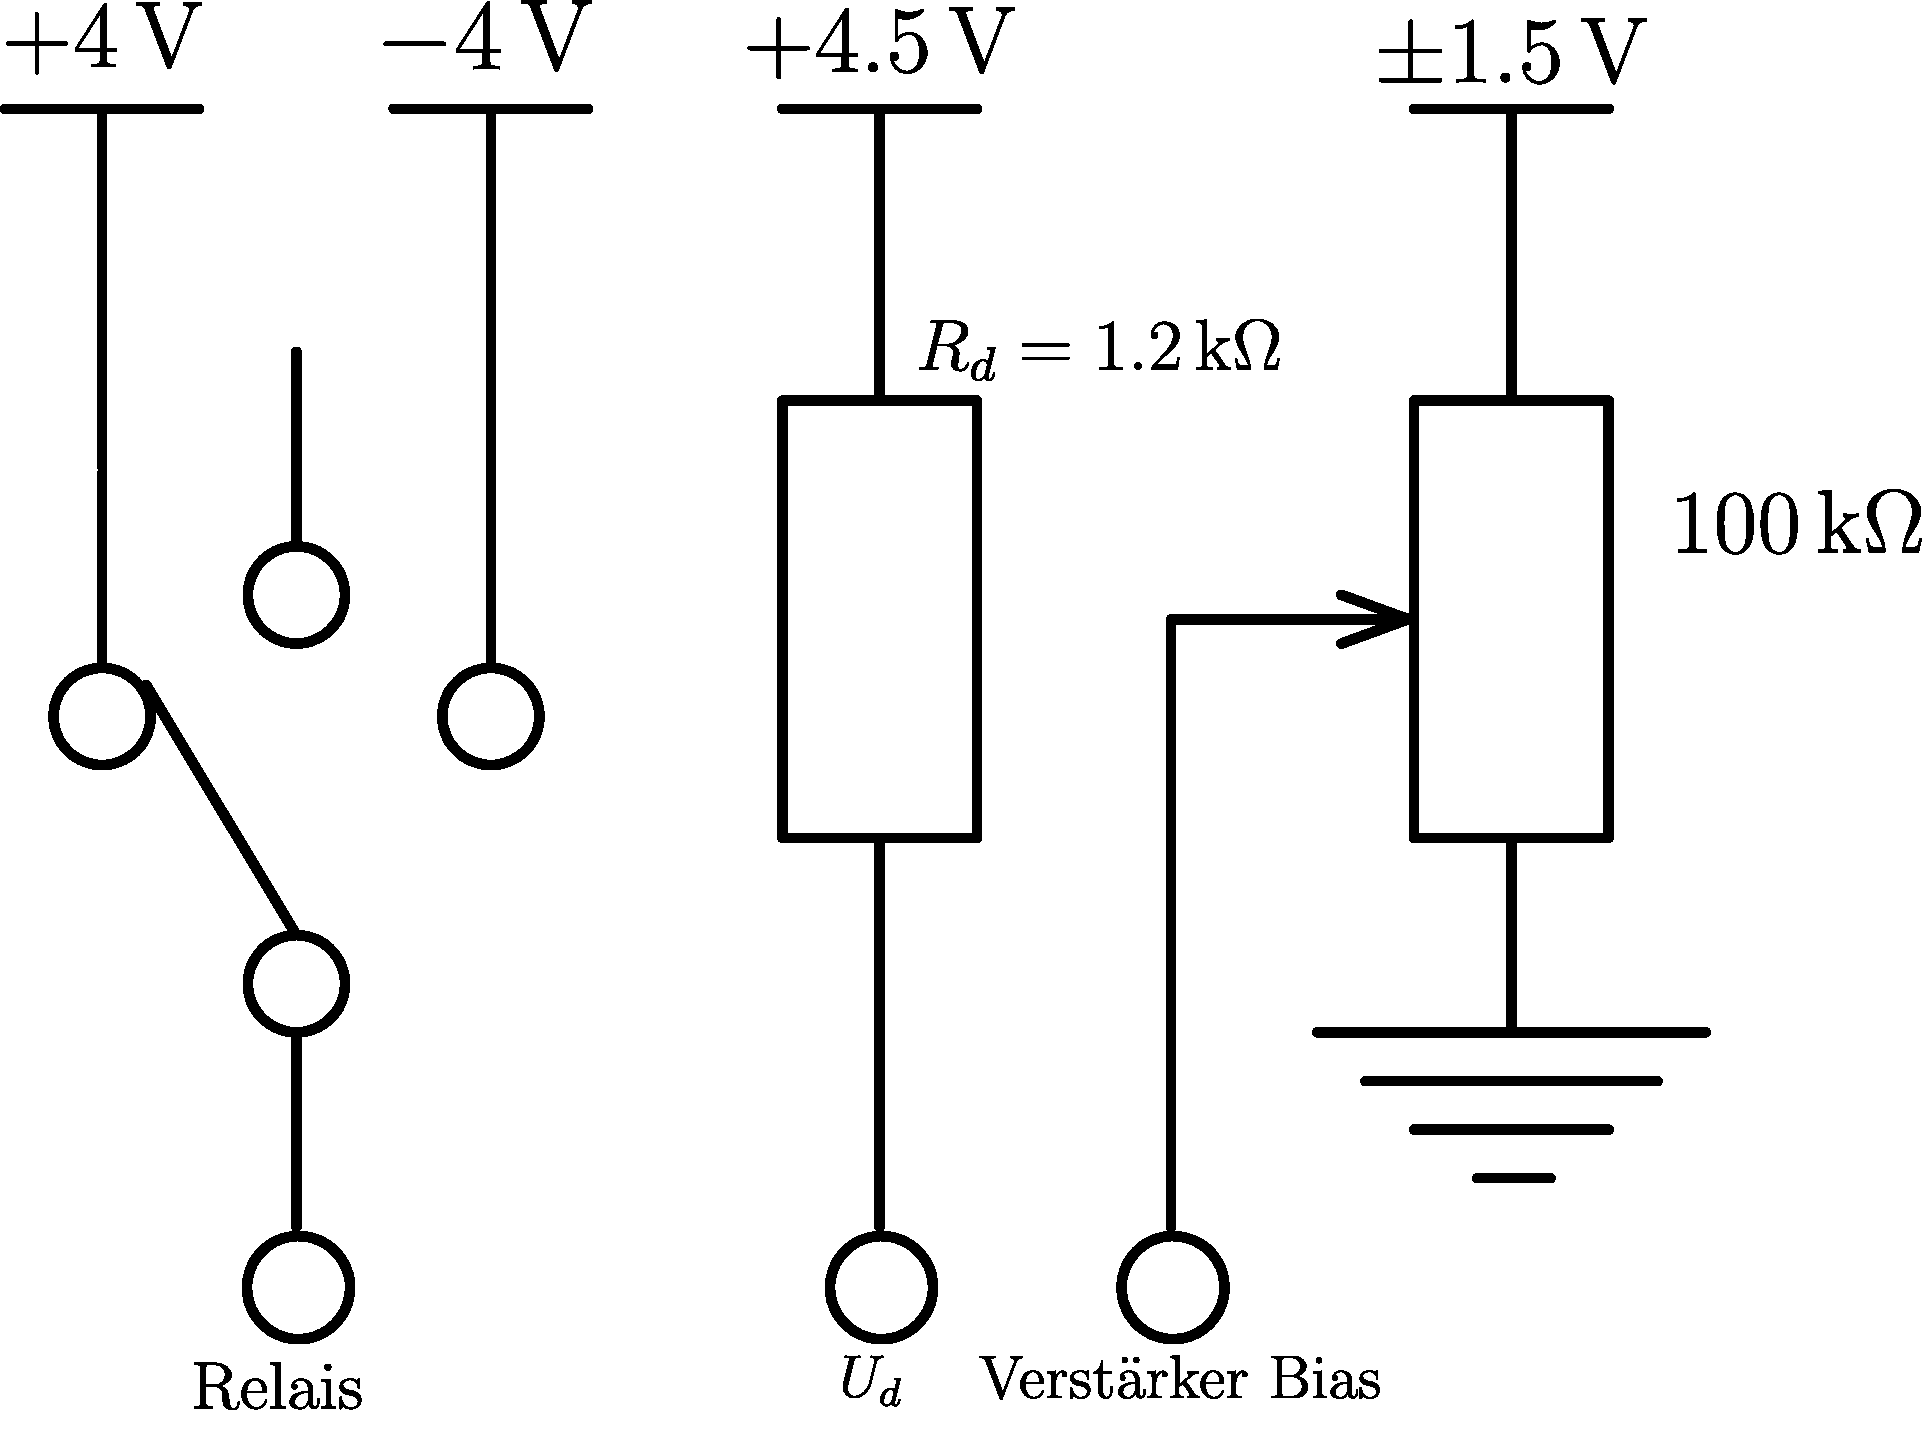
\includegraphics[width=0.5\textwidth]{./fig/Box.pdf}
\vspace{-0.5cm}
\caption{Schaltbild der warmen Elektronik mit einem dreistufigen Schalter zum schalten der Relais, dem Drainwiderstand des Verstärkers und einem Potentiometer um die Biasspannung am Gate des Verstärkers einzustellen.}
\label{fig:WarmeElektronik}
\end{center}
\end{figure}
Dazu muss der in Abb. \ref{sec:Ausleseelektronik} gezeigte Schaltplan um einen dummy detector ergänzt werden.
Dieser entspricht einer Kapazität zu Ground deren Größe gleich der Detektorkapazität $C_d$ ist.
Als Detektorkapazität wurden $C_d=\SI{30}{\pico\farad}$ verwendet, welche aus den Abmessungen des Detektors und der Elektrode bestimmt wurde.

Um die Handhabung der kalten Elektronik zu vereinfachen wurde die in Abbildung \ref{fig:WarmeElektronik} gezeigte warme Elektronik entwickelt.
Mit dem dreistufigen Kippschalter werden die Relais geschaltet.
Die Spannung $U_d$ und der Widerstand $R_d$ ist der Teil des Verstärkers, welcher in Abbildung \ref{fig:Amp} außerhalb des Kryostaten ist.
Mit den $\SI{\pm 1.5}{\volt}$ und dem $\SI{100}{\kilo\ohm}$ Potentiometer lässt sich die gewünschte Verstärker Biasspannung einstellen.
Um das Rauschen zu minimieren und um Rückkopplung über die Spannungsquelle zu vermeiden wird die Drainspannung und die Verstärker Biasspannung mit unabhängigen Batterien versorgt.
Die Spannungen zum Schalten der Relais werden mittels Generator aufgebracht.
Im Warmen befindet sich außerdem ein Oszilloskop, mit welchem das Ausgangssignal aufgenommen wird.
Außerdem befindet sich im Warmen ein Signalgenerator, welcher ein Signal einer bestimmten Frequenz simuliert um die Übertragungsfunktion zu bestimmen.
Die Detektor Biasspannung ist für die Funktionsweise der Elektronik unbedeutend und wird daher auf $\SI{0}{\volt}$ gesetzt.
In Abbildung \ref{fig:ElektronikBilder} sind Bilder der kalten Elektronik (oben Vorder- und Rückansicht) sowie der warmen Elektronik (unten) gezeigt.

Die Kühlung der kalten Elektronik findet mit flüssigem Stickstoff statt.
Dabei wird auf eine aufwendige Temperaturregelung verzichtet weshalb nur das Verhalten bei Raumtemperatur und Flüssigstickstoff Temperatur untersucht wird.
Schließlich befindet sich die kalte Elektronik in einem Faraday-Käfig um sie gegenüber elektromagnetischer Strahlung abzuschirmen.
Allerdings kann elektromagnetische Strahlung trotzdem über die Kabel der Spannungsversorgung und der Signalleitungen das Signal beeinflussen.
\begin{figure}[!t]
\begin{center}
\includegraphics[width=\textwidth]{./fig/ElektronikBilder.pdf}
\vspace{-0.5cm}
\caption{Bilder der warmen und kalten Elektronik.
Oben rechts: Rückseite der kalten Elektronik. Oben link: Vorderseite der kalten Elektronik.
Unten: Warme Elektronik im Gehäuse.}
\label{fig:ElektronikBilder}
\end{center}
\end{figure}
